\usepackage[dvipdfmx]{graphicx,xcolor}
\usepackage[top=20truemm,left=25truemm,right=25truemm]{geometry}
\usepackage{amsmath}
\usepackage{here}
\usepackage{comment}
\usepackage{url}
\usepackage{plistings}
\usepackage{tikz}
\usepackage[framemethod=tikz]{mdframed}

\renewcommand{\lstlistingname}{リスト}

\newcommand{\chuo}[1]{\multicolumn{1}{|c|}{#1}}
\newcommand{\inpt}[1]{\underline{#1}\,\setlength{\fboxsep}{1pt}\fbox{\small ↓}}

\lstdefinestyle{C}{
  language=C,
  basicstyle=\small\ttfamily,
  keywordstyle=\color[HTML]{0000E0},
  stringstyle=\color[HTML]{A31515},
  commentstyle=\upshape\color[HTML]{008000},
  frame=trbl,
  framesep=5pt,
  columns=[l]{fullflexible},
  numbers=left,
  xleftmargin=3zw,
  lineskip=-0.2ex,
  breaklines=true,
  showstringspaces=false,
  tabsize=4,
  keepspaces=true
}

\lstdefinestyle{text}{
  language=,
  basicstyle=\ttfamily,
  frame=trbl,
  framesep=5pt,
  columns=[l]{fullflexible},
  xleftmargin=3zw,
  lineskip=-0.2ex,
  showstringspaces=false,
  tabsize=4,
  keepspaces=true
}

\mdfsetup{
  skipabove=5pt,
  innertopmargin=10pt,
  innerbottommargin=10pt,
  roundcorner=10pt,
  font=\ttfamily
}


\begin{document}


\begin{titlepage}
  \title{\huge{シミュレーション} \\ \LARGE{---常微分方程式---}}
	\author{学籍番号:16426 \\ 4年 電子情報工学科 23番 \\ 福澤 大地}
	\date{提出日 : 2020年1月23日}
  \maketitle
\end{titlepage}


\section{目的}
常微分方程式の解法であるオイラー法、 ホイン法を応用して物理現象などを解析する。
連立微分方程式や高階微分方程式の数値解をプログラムを使用して解くことで目標の達成とする。


\section{開発環境}
プログラムの開発、実行を行った環境を表\ref{tb:kan}に示す。

\begin{table}[H]
  \centering
  \caption{開発環境}
  \label{tb:kan}

  \begin{tabular}{|l|l|}
    \hline
    CPU & Intel Core i5--7400 @ 3.0GHz \\ \hline
    メモリ & 8GB \\ \hline
    OS & Microsoft Windows 10 Home \\ \hline
    システム & 64bit \\ \hline
    コンパイラ & GCC 7.4.0 \\ \hline
  \end{tabular}
\end{table}


\section{課題6 : 生存競争モデル}
\subsection{課題内容}
式(\ref{seizon})に示す、生物の生存競争モデルの連立微分方程式をオイラー法で解くプログラムを作成する。

\begin{eqnarray}
  \begin{cases}
  \dfrac{dy_{1}}{dx} = ay_{1} - cy_{1} y_{2} & \\
  \dfrac{dy_{2}}{dx} -= by_2 + dy_{1} y_{2} &
  \label{seizon}
  \end{cases}
  \label{223759_6Jan19}
\end{eqnarray}

\subsection{プログラムリスト}
課題1のプログラムリストをリスト\ref{lst:kadai6}に示す。

\lstinputlisting[style=C,caption=課題6のプログラム,label=lst:kadai6]{code/kadai06-2.c}

\subsection{実行結果}
課題1の実行結果をリスト\ref{lst:kekka1}に示す。

\begin{lstlisting}[style=text,caption=課題1の実行結果,label=lst:kekka1]
i =  0, x = 0.0000000000000000, y1 = 10.0000000000000000, y2 = 10.0000000000000000
i =  1, x = 0.1000000000000000, y1 = 0.9999999999999996, y2 = 19.0000000000000000
i =  2, x = 0.2000000000000000, y1 = -0.7999999999999997, y2 = 19.0000000000000000
i =  3, x = 0.3000000000000000, y1 = 0.6399999999999999, y2 = 15.5800000000000001
i =  4, x = 0.4000000000000000, y1 = -0.2931200000000000, y2 = 15.0191199999999991
i =  5, x = 0.5000000000000000, y1 = 0.1178084454400000, y2 = 13.0769675545599995
i =  6, x = 0.6000000000000000, y1 = -0.0244684318832032, y2 = 11.9233285209712019
i =  7, x = 0.7000000000000000, y1 = 0.0022592401021203, y2 = 10.7018211537004380
i =  8, x = 0.7999999999999999, y1 = 0.0000673657607164, y2 = 9.6340568366820101
i =  9, x = 0.8999999999999999, y1 = 0.0000092017800292, y2 = 8.6707160535705672
i = 10, x = 0.9999999999999999, y1 = 0.0000021433558501, y2 = 7.8036524268156926
\end{lstlisting}

\subsection{考察}
まずはパラメータa, b, c, dの値が全て1の場合について
手計算で求めたオイラー法の答えを確認する。
例として、初期条件が$y_1(x_0)=10,y_2(x_0)=10,h=0.1$であるときの$y_1(x_1),y_2(x_1)$を求める.
手計算で求めた結果を式(\ref{eq:kadai6})に示す.

\begin{equation*}
\begin{split}
y_1(x_1)=&y_1(x_0)+ h\left\{ ay_{1}\left( x_{0}\right) -cy_{1}\left( x_{0}\right) y_{2}\left( x_{0}\right) \right\} \\
        =&10+0.1(1\times10-1\times10\times10)\\
        =&10-9=\underline{1}\\
y_2(x_1)=&y_2(x_0)+ h\left\{ -by_{1}\left( x_{0}\right) +dy_{1}\left( x_{0}\right) y_{2}\left( x_{0}\right) \right\} \\
=&10+0.1(-1\times10+1\times10\times10)\\
=&10+9=\underline{19}      
\end{split}
\label{eq:kadai6}
\end{equation*}

これは、リスト\ref{lst:kekka1}の結果と一致しているので、正しく計算が行えている。

次に変数$y_1,y_2$を縦軸、時間$x$を横軸としてプロットしたグラフを図\ref{graph_kadai5}に示す。

\begin{figure}[htbp]
\centering
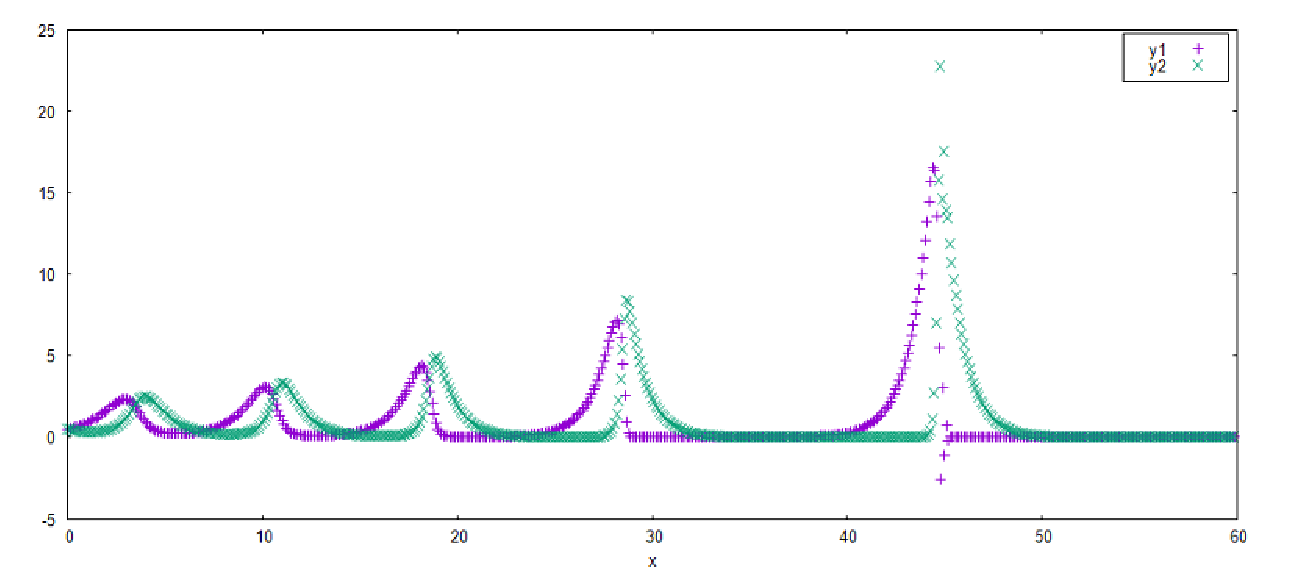
\includegraphics[scale=0.7]{./img/kadai5.eps}
\caption{生存競争モデル}
\label{graph_kadai5}
\end{figure}

生存競争モデルであるため$y_1$を被食者、$y_2$を捕食者として考えると、次のような循環があることがわかる.

\begin{enumerate}
 \item 被食者が増える。
 \item 捕食者が増える。
 \item 捕食者に食べられて被食者が減る。
 \item 被食者が少なくなったため,捕食者が減る。
 \item 捕食者が減ったため、被食者がまた増えて(1)に戻る。
\end{enumerate}

次に、初期条件を$y_1(0)=10,y_2(0)=0$とし、パラメータ$a,b,c,d$を変更した場合について考える。
パラメータの値を$a=1,b=1,c=0.01,d=0.01$とした場合のグラフを図\ref{5-1}に、
$a=0.01,b=1,c=1,d=0.01$とした場合のグラフを図\ref{5-2}に、
$a=1,b=0.01,c=0.01,d=1$とした場合のグラフを図\ref{5-3}に、
$a=b=c=d=1$とした場合のグラフを図\ref{5-4}に示す。

\begin{figure}[htbp]
\centering
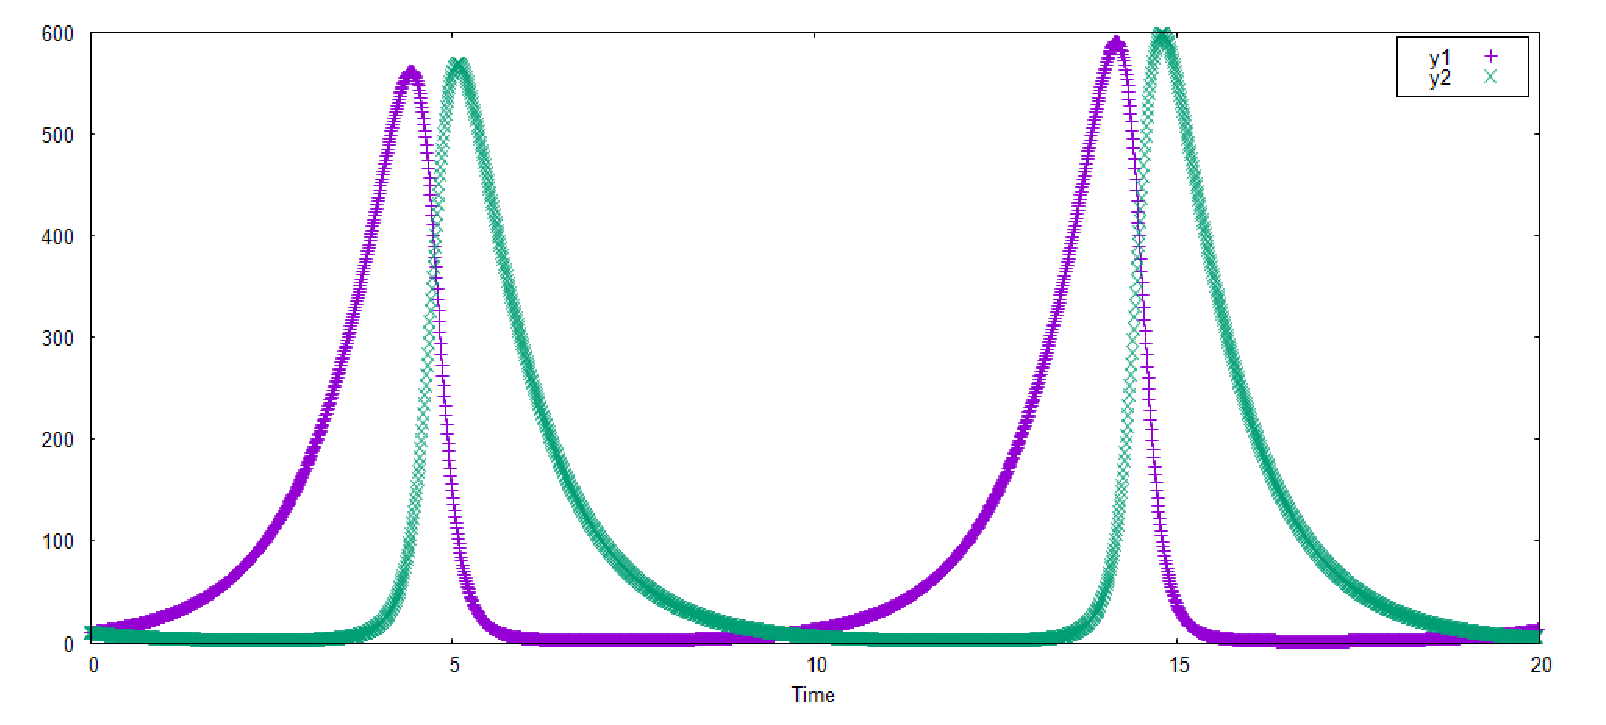
\includegraphics[scale=0.5]{./img/kadai5_1.eps}
\caption{$y_2<a/c,y_1<b/d$}
\label{5-1}
\end{figure}

\begin{figure}[htbp]
\centering
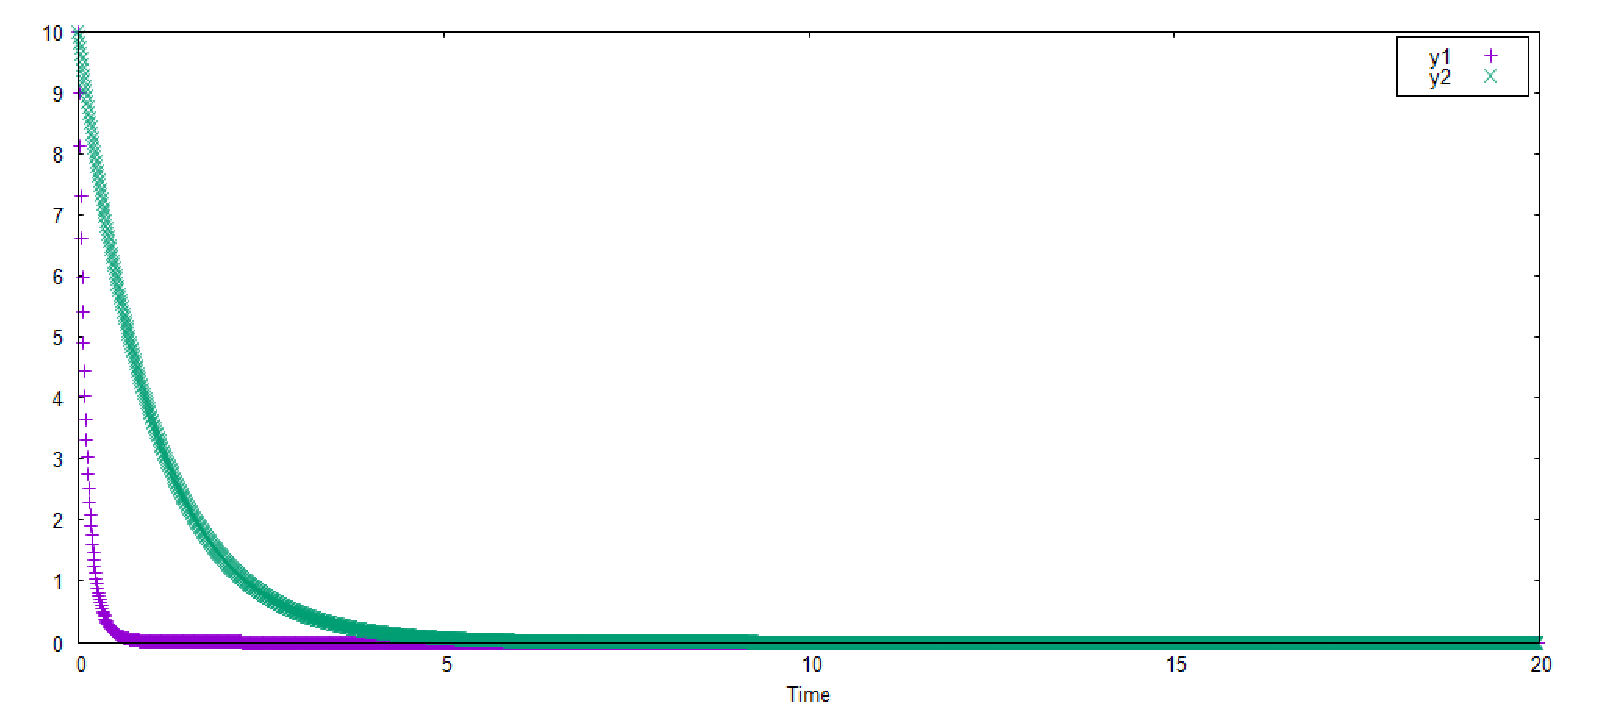
\includegraphics[scale=0.5]{./img/kadai5_2.eps}
\caption{$y_2>a/c,y_1<b/d$}
\label{5-2}
\end{figure}

\begin{figure}[htbp]
\centering
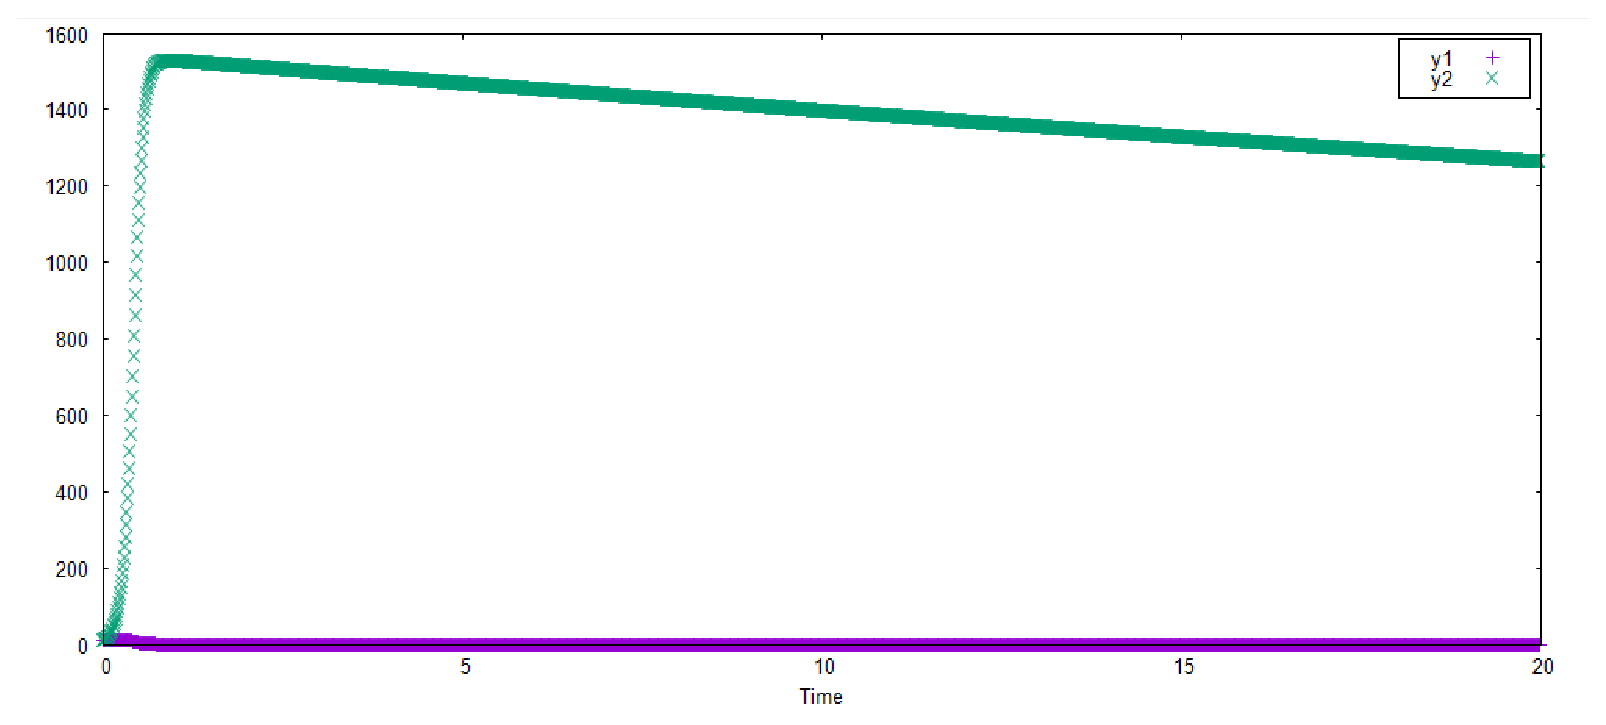
\includegraphics[scale=0.5]{./img/kadai5_3.eps}
\caption{$y_2<a/c,y_1>b/d$}
\label{5-3}
\end{figure}

\begin{figure}[htbp]
\centering
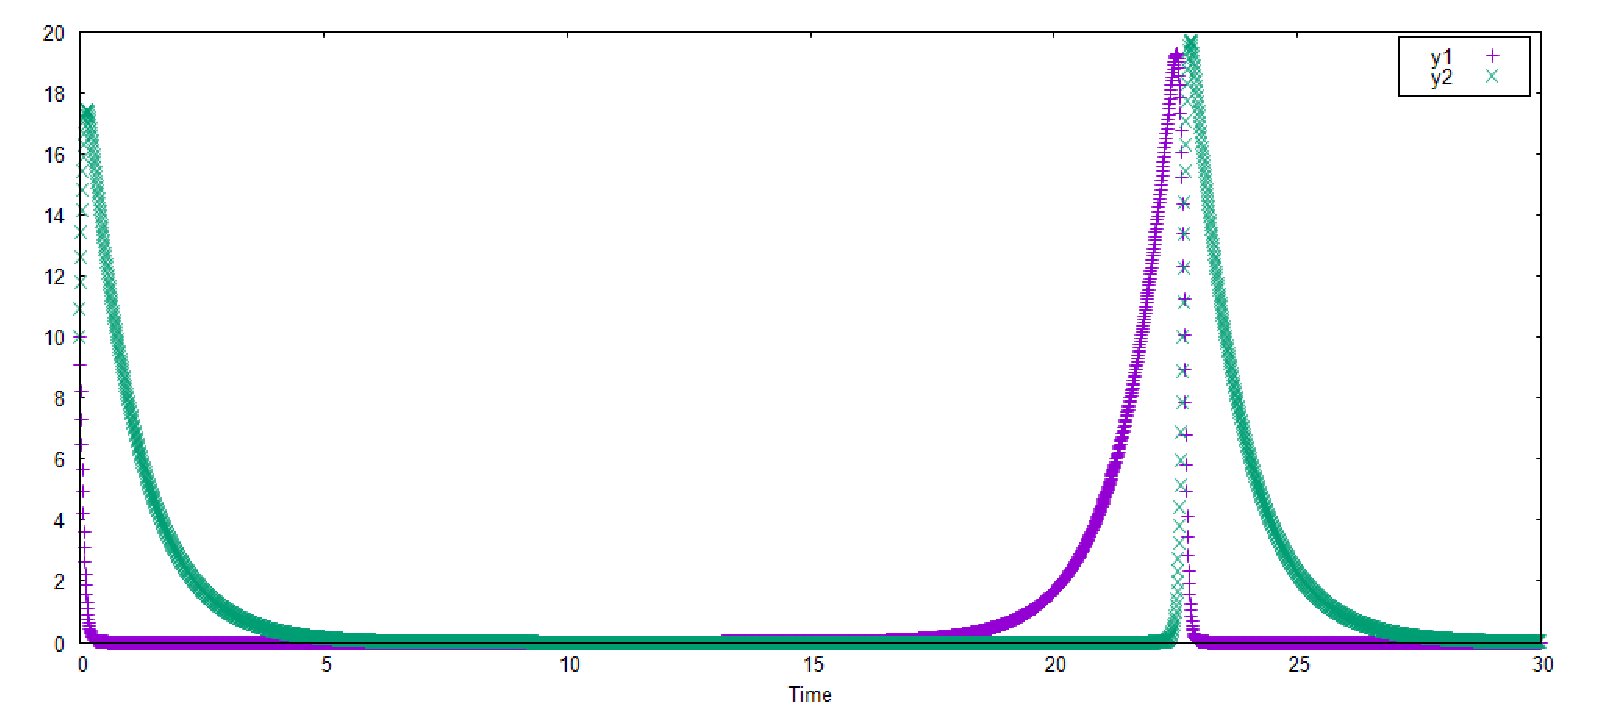
\includegraphics[scale=0.5]{./img/kadai5_4.eps}
\caption{$y_2>a/c,y_1>b/d$}
\label{5-4}
\end{figure}

図\ref{5-1}~\ref{5-4}と式(\ref{223759_6Jan19})より、パラメータ$a,b,c,d$には次のような意味があると考えられる.

\begin{itemize}
  \item $a$$\cdots$被食者の増えやすさ
  \item $b$$\cdots$捕食者の減りやすさ
  \item $c$$\cdots$捕食者の数と比例した被食者の減りやすさ
  \item $d$$\cdots$被食者の数と比例した捕食者の増えやすさ
\end{itemize}

図\ref{5-1}, \ref{5-4}では各パラメータのバランスが取れているため、前述した箇条書きのような循環が起こっている。
その一方で図\ref{5-2}, \ref{5-3}ではパラメータ同士のバランスが取れていないため、被食者の数が多くなり、
最終的にはどちらも絶滅してしまう。
図\ref{5-2}では$a$が小さく、$c$が大きいため、被食者が増えにくく減りやすくなる。
捕食者はパラメータ上では減りにくく増えにくいが、被食者が減りやすい状態においては捕食者も減りやすくなってしまう。
図\ref{5-3}では$b$が小さく$d$が大きいため、捕食者が増えやすく減りにくくなる。
被食者の数もパラメータ上では増やすく減りにくいので捕食者が一気に増加するが、被食者が減りすぎて捕食者は少しずつ少なくなっていく。
図\ref{5-2}とは異なり、捕食者が少しづつ減っているのはパラメータ$b$により減りにくくなっているためだと考えられる。


\section{課題7 : ニュートンの運動方程式}
式(\ref{newton1})に示す、ニュートンの運動方程式の高階微分方程式をオイラー法で解くプログラムを作成する。

\begin{eqnarray}
  \begin{cases}
mv'=-ky-lv&\\
y'= v&
 \label{newton1}
  \end{cases}\label{newton1}
\end{eqnarray}

\subsection{プログラムリスト}
課題7のプログラムリストをリスト\ref{lst:kadai7}に示す。

\lstinputlisting[style=C,caption=課題7のプログラム,label=lst:kadai7]{code/kadai07-2.c}

\subsection{実行結果}
課題7の実行結果をリスト\ref{lst:kekka7}に示す。

\begin{lstlisting}[style=text,caption=課題7の実行結果,label=lst:kekka7]
i =  0, t = 0.0000000000000000, y = 10.0000000000000000, v = 0.0000000000000000
i =  1, t = 0.1000000000000000, y = 10.0000000000000000, v = -2.0000000000000000
i =  2, t = 0.2000000000000000, y = 9.8000000000000007, v = -3.3999999999999999
i =  3, t = 0.3000000000000000, y = 9.4600000000000009, v = -4.3399999999999999
i =  4, t = 0.4000000000000000, y = 9.0260000000000016, v = -4.9299999999999997
i =  5, t = 0.5000000000000000, y = 8.5330000000000013, v = -5.2561999999999998
i =  6, t = 0.6000000000000000, y = 8.0073800000000013, v = -5.3859399999999997
i =  7, t = 0.7000000000000000, y = 7.4687860000000015, v = -5.3716340000000002
i =  8, t = 0.7999999999999999, y = 6.9316226000000016, v = -5.2539010000000008
i =  9, t = 0.8999999999999999, y = 6.4062325000000016, v = -5.0640552200000011
i = 10, t = 0.9999999999999999, y = 5.8998269780000010, v = -4.8260851540000012
\end{lstlisting}

\subsection{考察}
初期条件を$t=2$のとき$y=10,y'=0$として計算を行うプログラムを
ソースコード\ref{neweu}に示す.$m=1,k=2,l=3$とした場合の実行結果を次に示す.
\begin{breakitembox}[l]{課題6-1の結果}
\begin{verbatim}

t: 0.1 ,y: 10.0 ,v: -2.0

\end{verbatim}
\end{breakitembox}
手計算で求めた結果を次に示す.$y,v$をそれぞれtの関数$y(t),v(t)$とした.
\begin{equation*}
\begin{split}
v(0.1)=& v(0) + h(-2y-3v)\\
=& 0+0.1(-2\times-3\times0)\\ 
=& \underline{-2}\\
y(0.1)=& y(0)+v\\
=&10 + 0 = \underline{10}
\end{split}
\end{equation*}

プログラムの実行結果と一致したため,正しく計算できていることがわかる.初期条件を
$m=1,k=1,l=0$と変更した場合のプログラムをソースコード\ref{neweu2}に示す.
\lstinputlisting[caption=課題6-2のプログラム,label=neweu2]{./program/kadai6/ka2.py}
\begin{figure}[htbp]
\centering
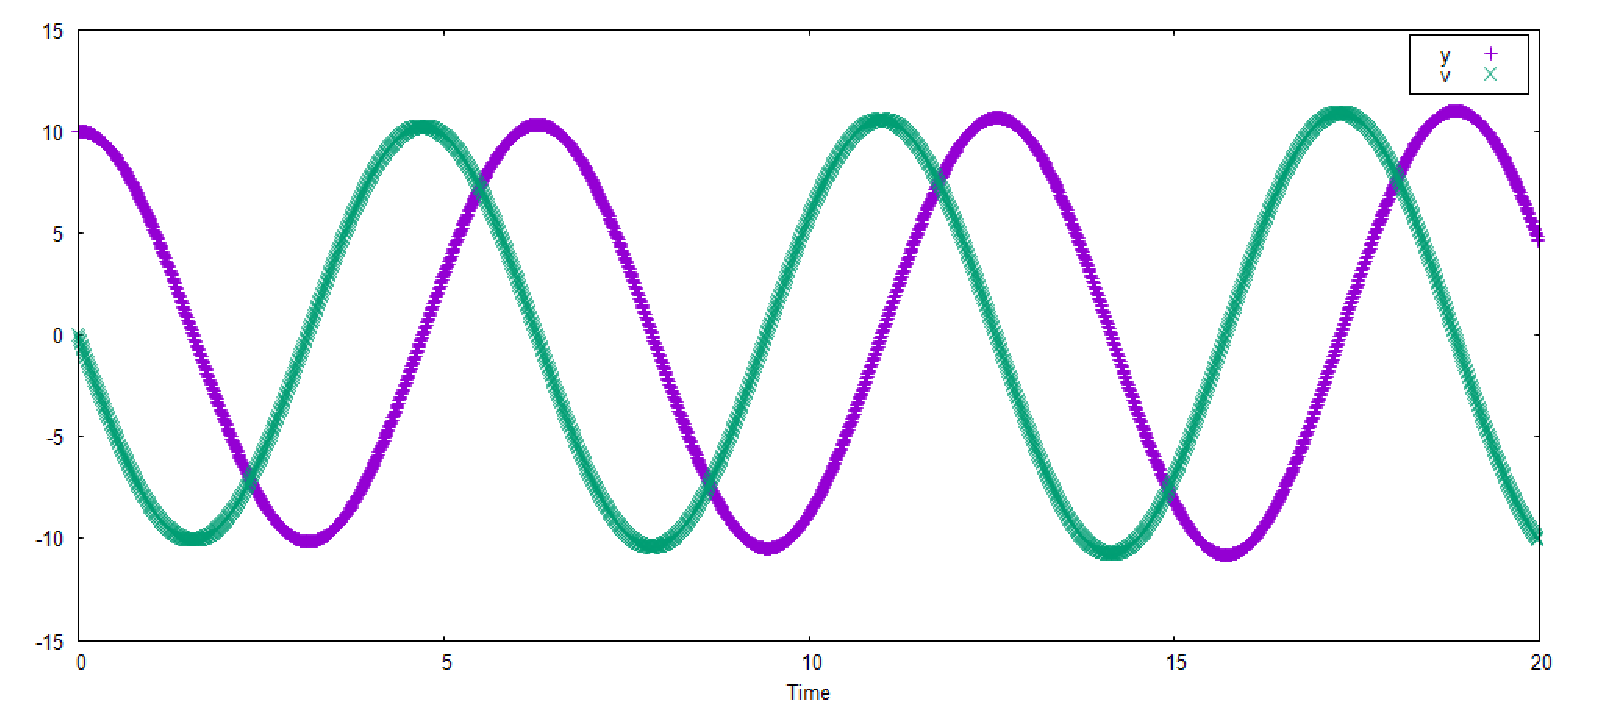
\includegraphics[scale=0.5]{./img/kadai6_1mkl_110.eps}
\caption{初期条件$m=1,k=1,l=0$}
\label{101837_6Jan19}
\end{figure}
\begin{figure}[htbp]
\centering
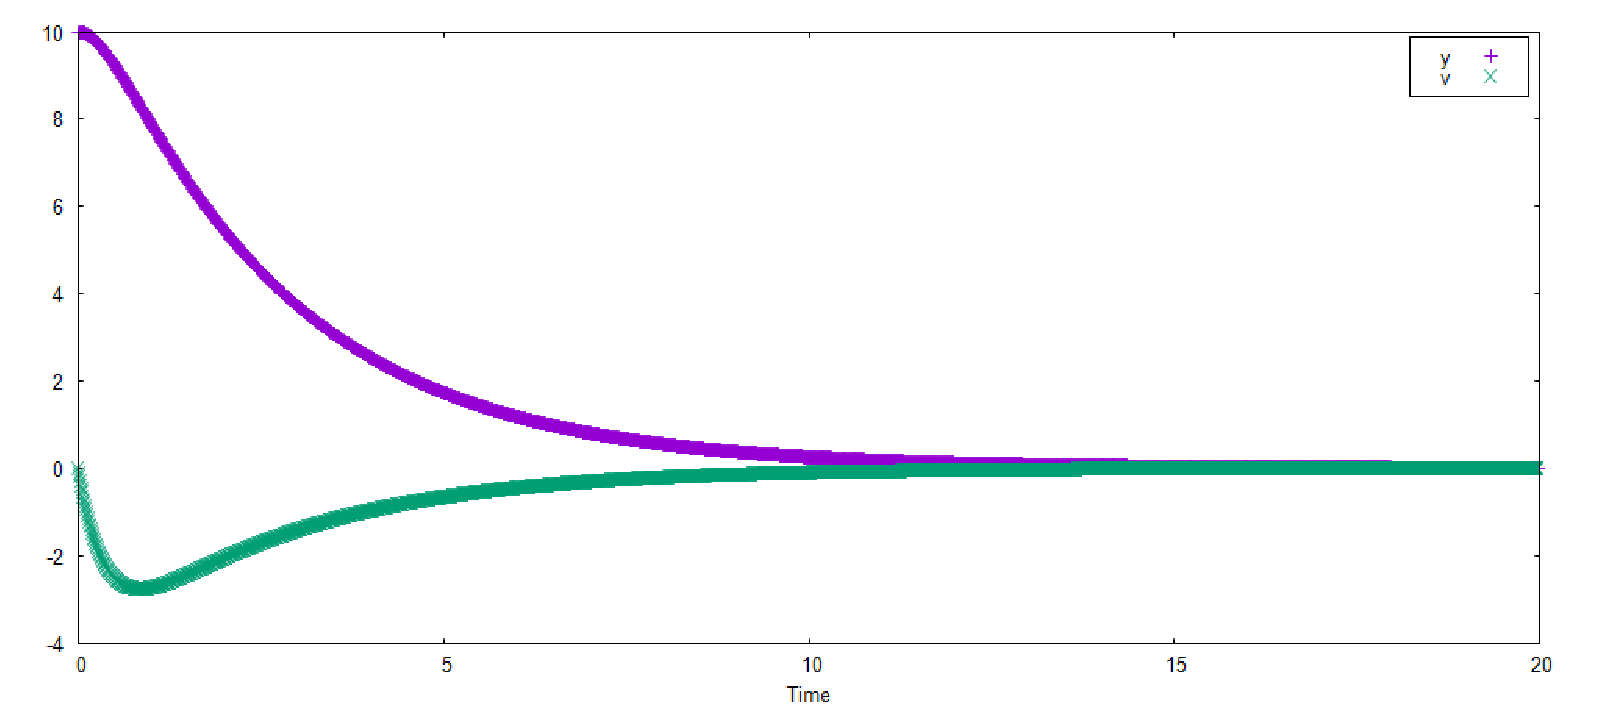
\includegraphics[scale=0.5]{./img/kadai6_2mkl_113.eps}
\caption{初期条件$k=1,l=3$}
\label{mkl113}
\end{figure}
\begin{figure}[htbp]
\centering
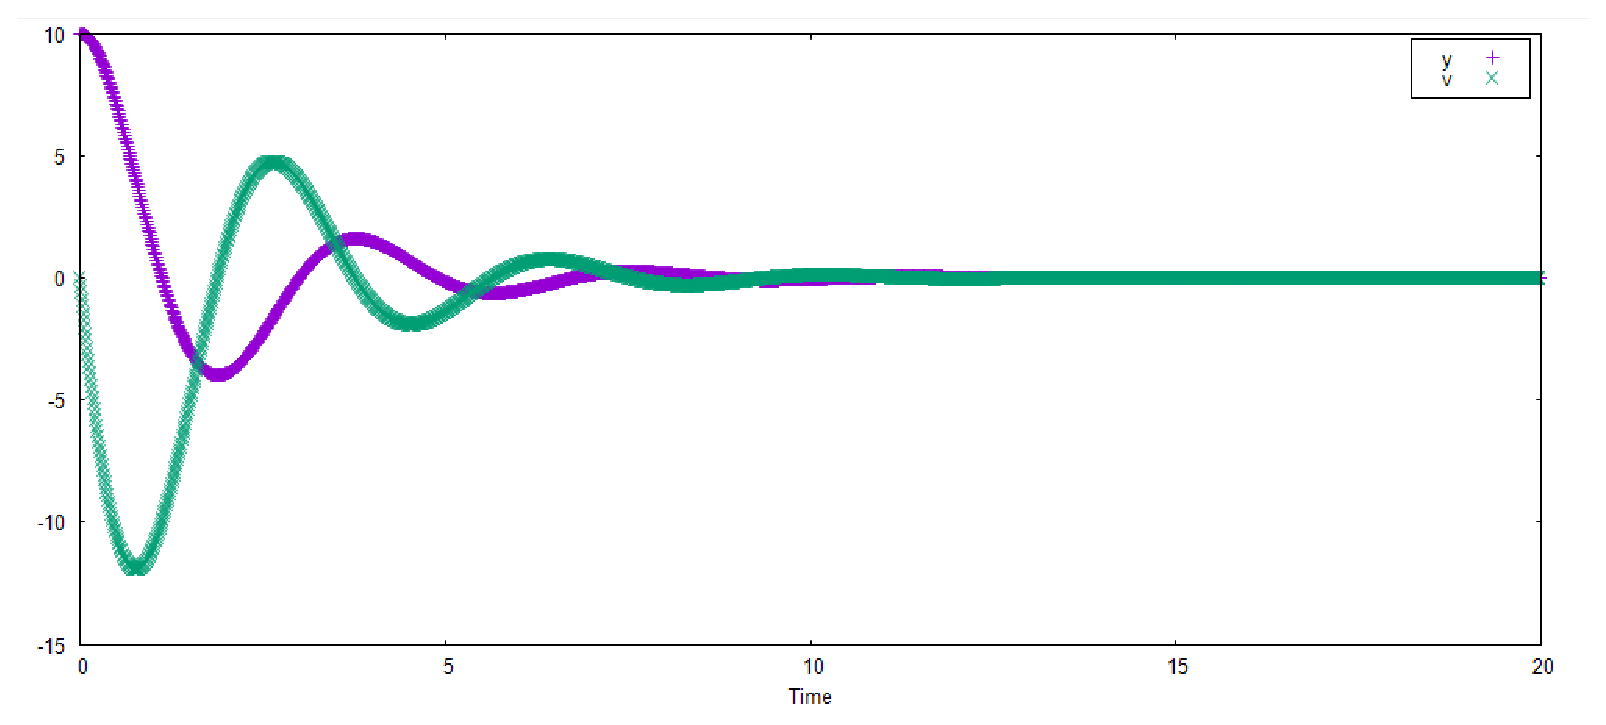
\includegraphics[scale=0.5]{./img/kadai6_3mkl_131.eps}
\caption{初期条件$k=3,l=1$}
\label{mkl131}
\end{figure}

実行結果をテキストファイルに出力し,グラフにプロットしたものを図\ref{101837_6Jan19}に
示す.図\ref{101837_6Jan19}は$l=0$であるため,単振動になっている.次に,初期条件
$k,l$を変更した場合のグラフを図\ref{mkl113},\ref{mkl131}に示す.
3つのグラフからばね定数を示す$k$が$y,v$の振動のしやすさに,摩擦係数の
$l$が振動のしにくさに関連していることがわかる.
そのため図\ref{mkl113}は$l$が大きく,振動が止まっている.図\ref{mkl131}は
$k$が大きいため図\ref{mkl113}よりは振動するが,$l=1$であるため振動が止まる.
%%%%%%%%%%%%%%%%%%%%%%%%%%%%%%%%%%%%%%%%%%%%%%%%%%%%%%%%%%%%
\section{課題7:RLC共振回路}
RLC共振回路の微分方程式
\begin{equation*}
\frac{dV}{dt^2}+\frac{R}{L}\frac{dC}{dt}+\frac{V}{LC}=0
\end{equation*}
をルンゲクッタ法によって解くプログラムをソースコード\ref{7-1}に示す.
課題5,6と同様に電流を表す変数$I=dV/dt$を導入して,
式(\ref{sikiRLC})のように2式に展開して計算を行う.
初期条件は$t=0$のとき,$V=E,dV/dt=0$とし,パラメータは$
C=0.3[nF],L=10[mH],E=1[V]$とした.
\begin{eqnarray}
  \begin{cases}
\frac{dV}{dt}=I&\\
\frac{dI}{dt}=-\frac{R}{L}I-\frac{V}{LC}&
 \label{sikiRLC}
  \end{cases}
\end{eqnarray}
\lstinputlisting[caption=課題7のプログラム,label=7-1]{./program/kadai7/ni.py}
ソースコード\ref{7-1}を実行すると,$R=0,3,6,9,2\sqrt{L/C}$それぞれについて
計算した結果がファイルに出力される.実行結果のデータをプロットした
グラフを図\ref{r0}~\ref{rsqr}に示す.図\ref{r0}より刻み幅は0.01が減衰しない刻み幅であることがわかった.
\begin{figure}[htbp]
\centering
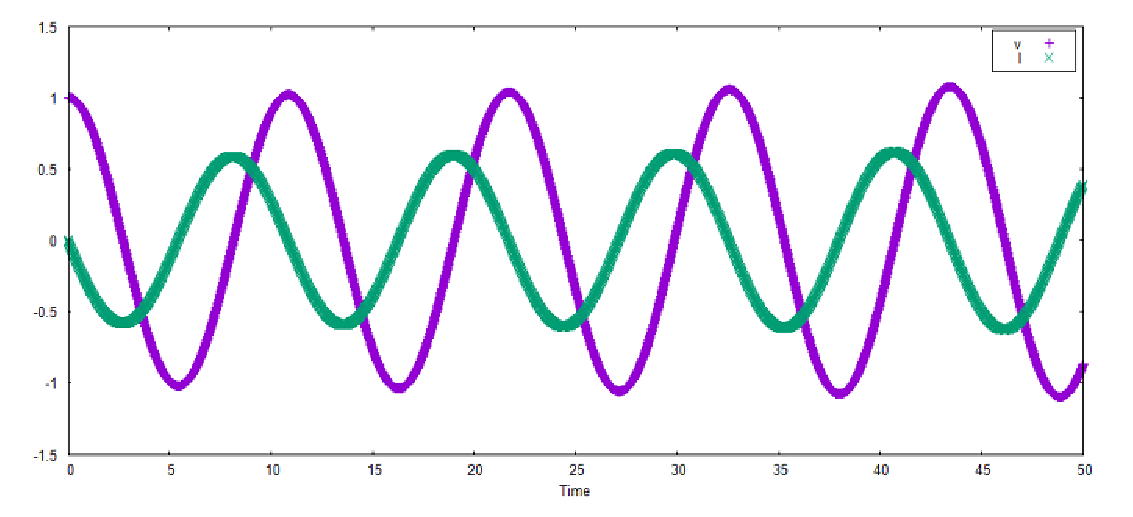
\includegraphics[scale=0.7]{./img/kadai7_R0.eps}
\caption{$R=0$}
\label{r0}
\end{figure}
\begin{figure}[htbp]
\centering
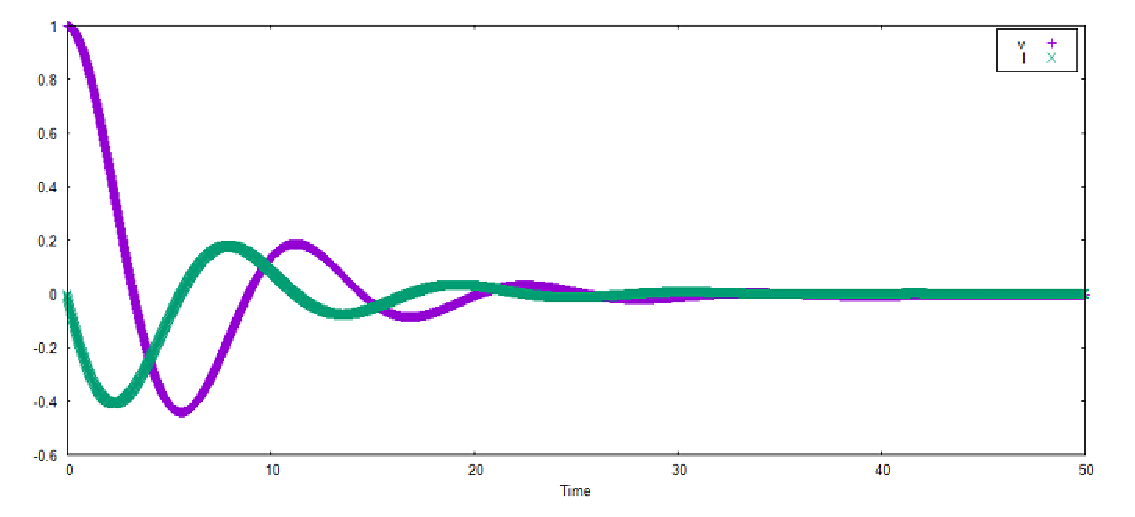
\includegraphics[scale=0.7]{./img/kadai7_R3.eps}
\caption{$R=3$}
\label{r3}
\end{figure}
\begin{figure}[htbp]
\centering
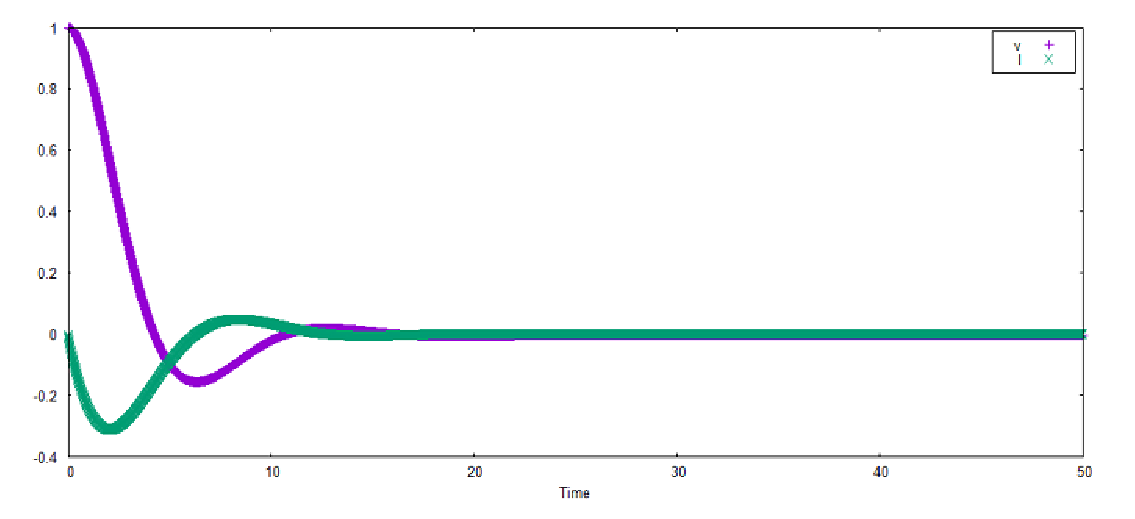
\includegraphics[scale=0.7]{./img/kadai7_R6.eps}
\caption{$R=6$}
\label{r6}
\end{figure}
\begin{figure}[htbp]
\centering
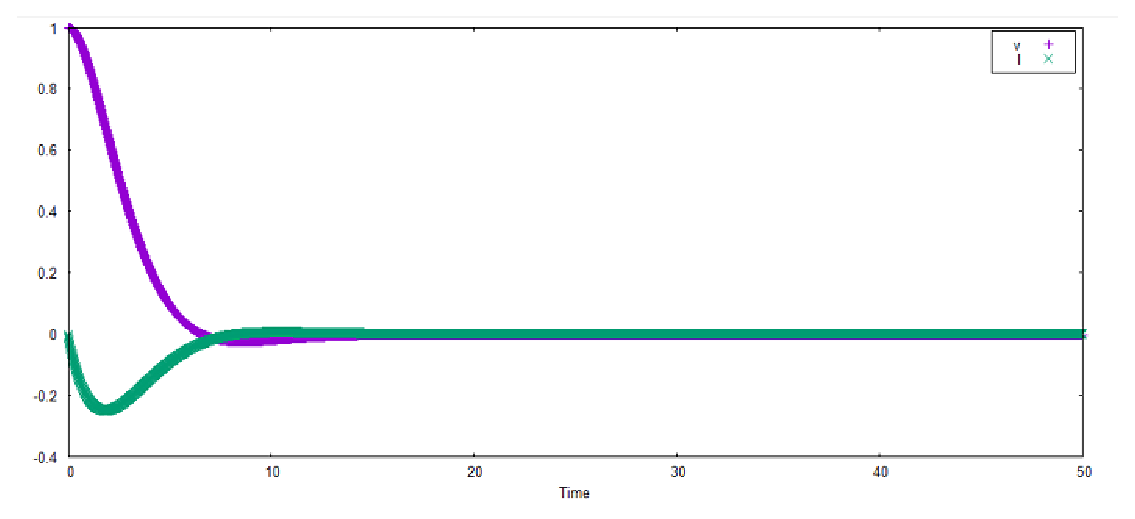
\includegraphics[scale=0.7]{./img/kadai7_R9.eps}
\caption{$R=9$}
\label{r9}
\end{figure}
\begin{figure}[htbp]
\centering
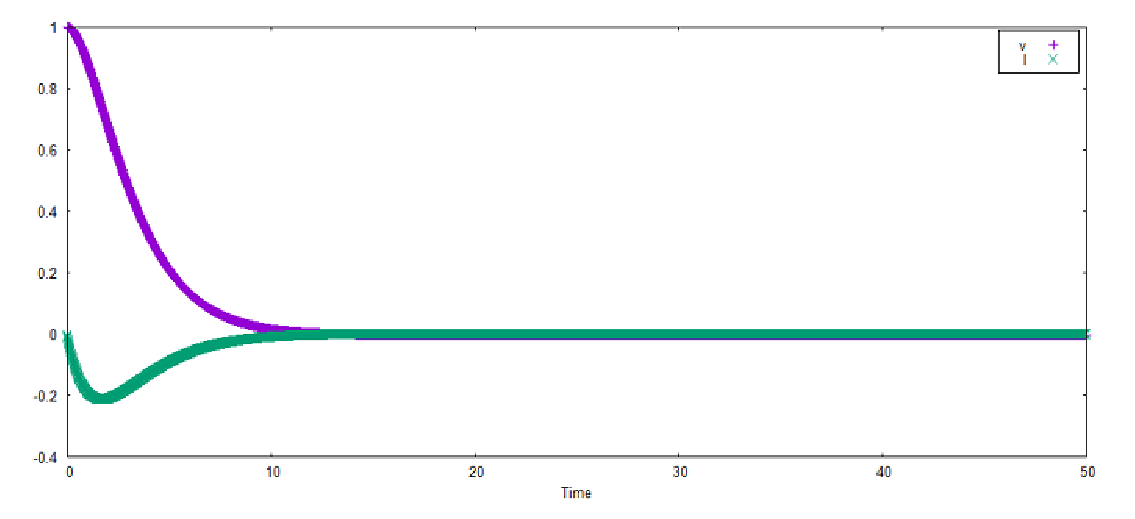
\includegraphics[scale=0.7]{./img/kadai7_sqr.eps}
\caption{$R=2\sqrt{L/C}$}
\label{rsqr}
\end{figure}

図\ref{r0}~\ref{rsqr}より$R$が大きければ大きいほど
振動が収まりやすくなっているため,$R$は振動のしやすさに
関連していることがわかる.これは$R$が抵抗の値であり,$R$と$V,I$が反比例
の関係にあるためだと考えられる.
%%%%%%%%%%%%%%%%%%%%%%%%%%%%%%%%%%%%%%%%%%%%%%%%%%%%%%%%%%%%
\section{課題8:ローレンツ力}
ローレンツ力とは荷電粒子が磁場から受ける力のことである.
速度$v$で運動している電荷$q$の荷電粒子が磁場$B$から受けるローレンツ力は
$qvB$であるため,運動方程式は式(\ref{siki8-1})のように表せる.ここで$x$を荷電粒子の変位,
$m$を荷電粒子の質量とする.
\begin{equation}
m\frac{d^2x}{dt^2}=q\frac{dx}{dt}B
\label{siki8-1}
\end{equation}

数値計算では式(\ref{siki8-2})をホイン法を用いて計算する.
\begin{eqnarray}
  \begin{cases}
\frac{dx}{dt}=v&\\
\frac{dv}{dt}= \frac{qvB}{m}&
 \label{siki8-2}
  \end{cases}
\end{eqnarray}
\lstinputlisting[caption=課題8-1のプログラム,label=ka8-1]{./program/kadai8/one.py}

パラメータを$qB/m=2.0$,
初期条件を$t=0$において$x=0,v=1$としてソースコード\ref{ka8-1}
を実行する.$x,v$の解析解はプログラムと同様の初期条件で
次のように求められる.$x$の解析解は$v$
の解析解を式(\ref{siki8-2})の$x$に関する式の右辺に代入することで得られる.
\begin{equation*}
\begin{split}
&\int \frac{1}{v}dv=\dfrac{qB}{m}\int_{} dt\\
&\log \left| v\right| =\dfrac{qB}{m}t+C\\
&v=Ce^{\frac{qB}{m}t}=e^{\frac{qB}{m}t}=\underline{e^{2t}}\\
&\int dx=\int_e^{\frac{qB}{m}t} dt\\
&x=\frac{m}{qB}e^{\frac{qB}{m}t}+C=\frac{m}{qB}(e^{\frac{qB}{m}t}-1)=\underline{\frac{1}{2}(e^{2t}-1)}
\end{split}
\end{equation*}
\begin{figure}[htbp]
\centering
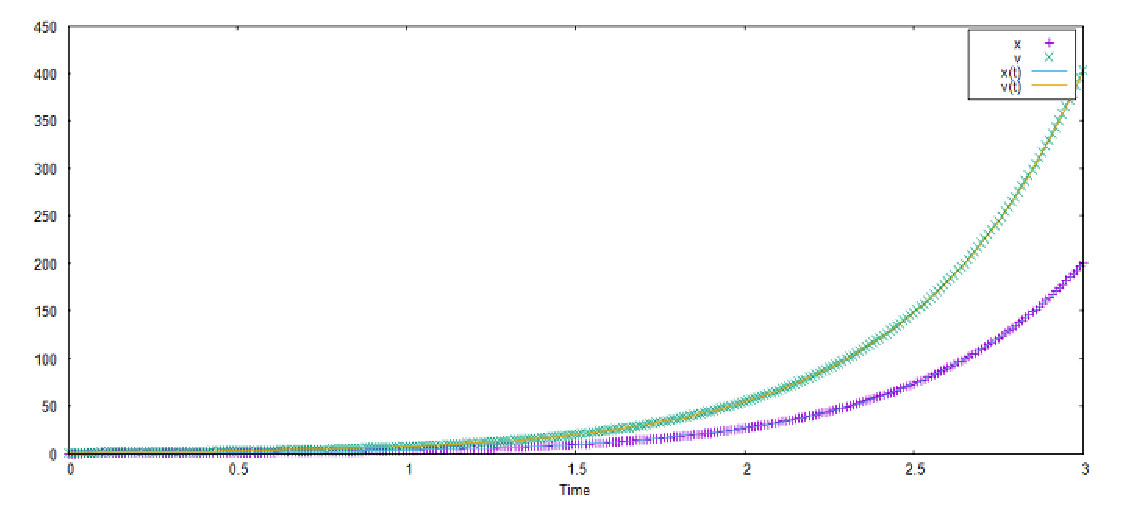
\includegraphics[scale=0.7]{./img/kadai8-1.eps}
\caption{$x(0)=0,v(0)=1$}
\label{kadai8-1}
\end{figure}

ソースコード\ref{ka8-1}を実行した結果と解析解をプロットしたグラフを図\ref{kadai8-1}
に示す.$x(t),v(t)$が解析解である.値がほぼ一致しているため,正しく計算できている
ことがわかる.
次に$xy$平面で荷電粒子が運動する場合について考える.
変位の$x$成分を$x$,$y$成分を$y$とし,速度も同様に成分ごとに$v_x,v_y$とすると,
運動方程式は式(\ref{siki8-2})のように表せる.
\begin{equation}
\begin{split}
m\dfrac {dv_{x}}{dt}=&qv_{y}B\\
m\dfrac {dv_{y}}{dt}=&-qv_{x}B
\label{siki8-2}
\end{split}
\end{equation}

磁場$B$の方向は荷電粒子の運動平面と直交しているため,磁場は
荷電粒子に対して仕事をしない.このためx,y平面の運動エネルギーは
保存する.よって式(\ref{siki8-3})が成り立ち,${v_x}^2+{v_y}^2$は一定である.
\begin{equation}
\frac{1}{2}m{v_x}^2+\frac{1}{2}m{v_y}^2=一定
\label{siki8-3}
\end{equation}

式(\ref{siki8-2})を$x,y$について,それぞれホイン法で計算するプログラム
をソースコード\ref{ka8-2}に示す.初期条件は$t=0.0$のとき,$x=0.1.y=0.0,
v_x=0.0,v_y=0.1$,パラメータは$q=m=1.0$とした場合に$B$を変化させて計算を行う.
$B=1,2,10$のときの計算結果をプロットしたグラフを図\ref{8b1}~\ref{8b10}に示す.
\lstinputlisting[caption=課題8-2のプログラム,label=ka8-2]{./program/kadai8/two.py}

誤差はそれぞれ次のようになった.$t=0の{v_x}^2+{v_y}^2の値を
V_0,nステップ後の{v_x}^2+{v_y}^2の値をV_nとすると,
誤差は(V_n - V_0)/V_0$で求められる.
$B$が大きくなればなるほど誤差が大きくなっており,エネルギー保存則が成り立たなくなっている
ことがわかる.図\ref{8b1}~\ref{8b10}からも$B$が大きくなればなるほどエネルギー保存則
が成り立たなくなり,より外側に軌道を描くようになっていることがわかる.さらに
$B$が大きいほど円軌道が小さくなっており,$B$と円軌道の大きさは反比例の関係にあると考えられる.
\begin{breakitembox}[l]{$B=1,3,10$のときの誤差}
    \begin{verbatim}

B: 1 ,誤差: 0.0092120809404796
B: 3 ,誤差: 0.08735045022264068
B: 10 ,誤差: 1.4792738717251592
 \end{verbatim}
\end{breakitembox}
\begin{figure}[htbp]
\centering
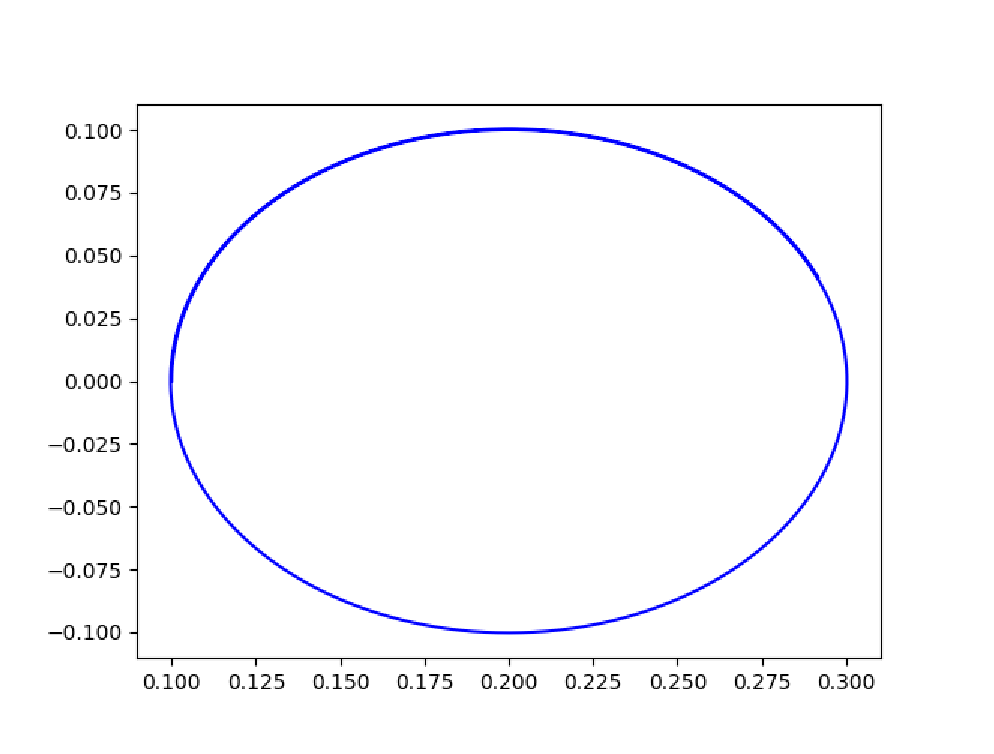
\includegraphics[scale=0.8]{./img/ka8_b1.eps}
\caption{$B=1$}
\label{8b1}
\end{figure}
\begin{figure}[htbp]
\centering
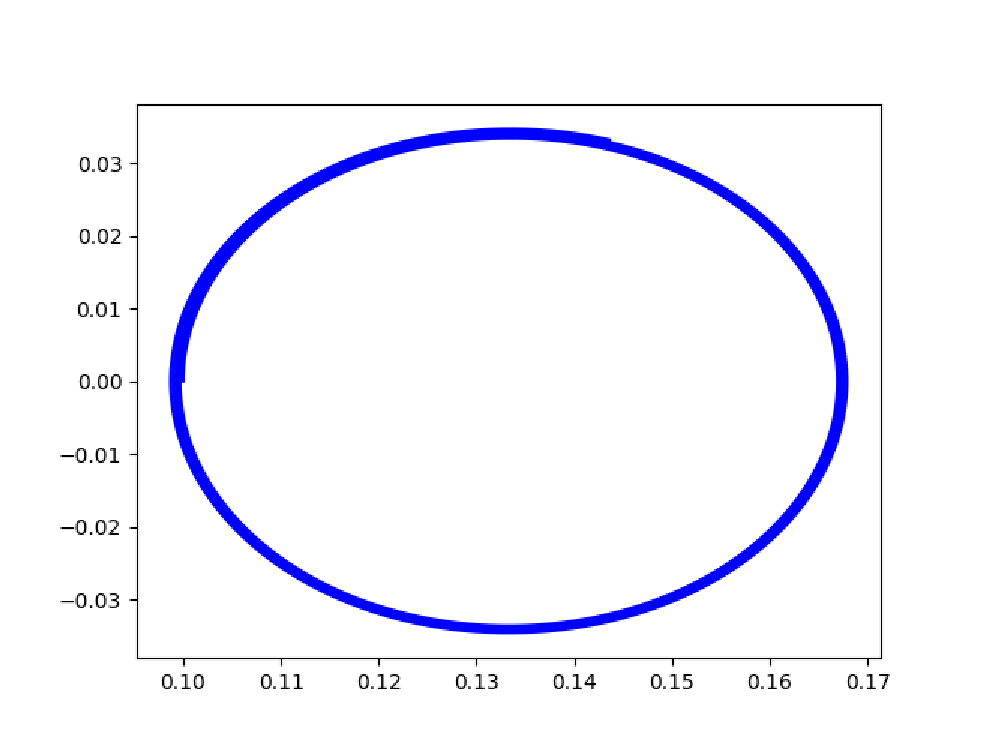
\includegraphics[scale=0.8]{./img/ka8_b3.eps}
\caption{$B=3$}
\label{8b3}
\end{figure}
\begin{figure}[htbp]
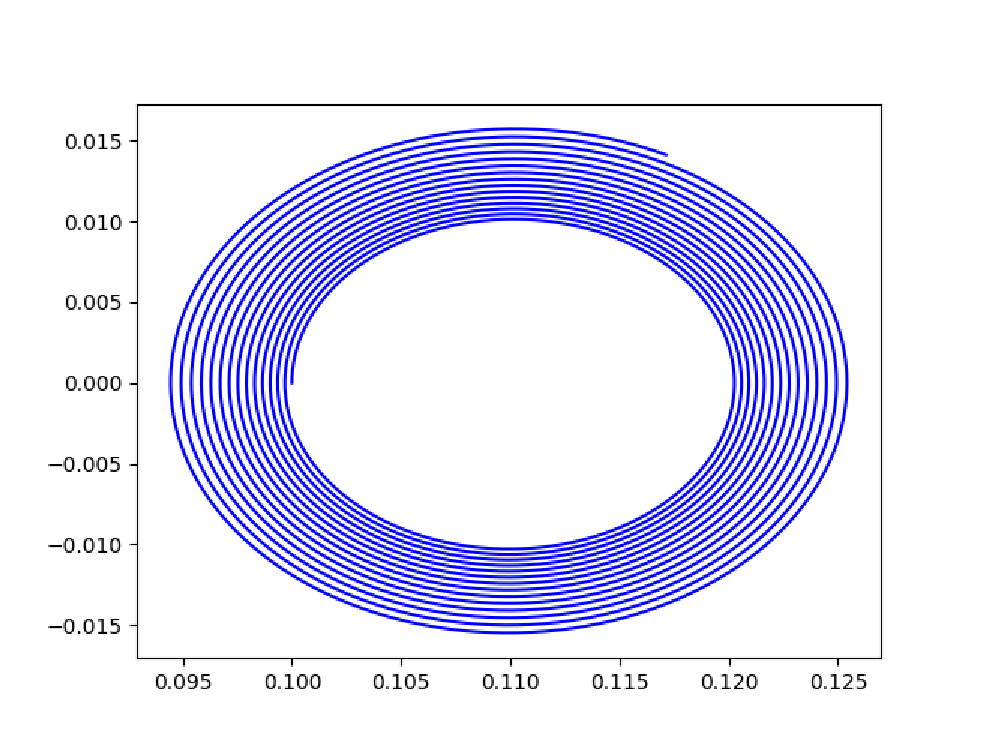
\includegraphics[scale=0.8]{./img/ka8_b10.eps}
\centering
\caption{$B=10$}
\label{8b10}
\end{figure}

%\lstinputlisting[caption=,label=]{}

%\begin{figure}[htbp]
%\centering
%\includegraphics[scale=1]{.eps}
%\caption{}
%\label{}
%\end{figure}


%参考文献
%\cite{}
%\begin{thebibliography}{9}
% \bibitem{harris} springs of c
%  \bibitem{susan} 
%\end{thebibliography}

\end{document}